%                                                                 aa.dem
% AA vers. 8.2, LaTeX class for Astronomy & Astrophysics
% demonstration file
%                                                       (c) EDP Sciences
%-----------------------------------------------------------------------
%
%\documentclass[referee]{aa} % for a referee version
%\documentclass[onecolumn]{aa} % for a paper on 1 column  
%\documentclass[longauth]{aa} % for the long lists of affiliations 
%\documentclass[rnote]{aa} % for the research notes
%\documentclass[letter]{aa} % for the letters 
%\documentclass[bibyear]{aa} % if the references are not structured 
% according to the author-year natbib style

%
\documentclass{aa}  

%
\usepackage{graphicx}
%%%%%%%%%%%%%%%%%%%%%%%%%%%%%%%%%%%%%%%%
\usepackage{txfonts}
%%%%%%%%%%%%%%%%%%%%%%%%%%%%%%%%%%%%%%%%
\usepackage{hyperref}
\hypersetup{pdfborder=0 0 0, colorlinks=true, linkcolor=black, urlcolor=blue,
citecolor=black}
% To add links in your PDF file, use the package "hyperref"
% with options according to your LaTeX or PDFLaTeX drivers.
%
\newcommand{\Sun}[0]{\ensuremath{_{\odot}}}
\newcommand{\mytilde}{\raise.17ex\hbox{$\scriptstyle\mathtt{\sim}$}}
\begin{document} 


   \title{Simulating Ultra Compact Dwarf Galaxies with AMUSE}

   \subtitle{Computational Astrophysics (CA) assignment one}

   \author{T. Halbesma (1603221)
          \inst{1}
          \and
          S. Sultan (1617451)\inst{2}
          }

   \institute{Anton Pannekoek Instituut (API), University of Amsterdam,
              Science Park 904, 1098 XH Amsterdam 
              \email{timo.halbesma@student.uva.nl}
         \and
             Informatics Institute, Section Computational Science, University of Amsterdam,
             Science Park 904, 1098 XH Amsterdam 
             \email{shabaz.sultan@student.uva.nl}
             }

   %\date{Received September 15, 1996; accepted March 16, 1997}

% \abstract{}{}{}{}{} 
% 5 {} token are mandatory
 
  \abstract
  % context heading (optional)
  % {} leave it empty if necessary  
   {To investigate the computational nature of different N-Body algorithms
   available in the AMUSE framework, to model interactions that occur 
   when galaxies collide in orde to obtain the bound particles and the total
   post-encounter bound mass in the galaxy.}
  % aims heading (mandatory)
   {To investigate the performance of different 
   N-Body algorithms, to simulate an Ultra Compact Dwarfs galaxies in an orbit around
   a Black Hole (possibly other Galaxies such as the Milky Way).}
  % methods heading (mandatory)
   {We have used a three different N-Body integrators to calculate the gravity in a galaxy:
   a predictor corrector algorithm (Hermite), a direct approx. symplectic algorithm (Huayno),
   and a tree based algorithm (BHTree).}
  % results heading (mandatory)
   {It is shown that the BHTree algorithm has the most favoured time complexity
   of $O(n \log n)$ as compared to $O(n^2)$ for Huayno and Hermite, the
   relative energy error will increase as the time step of the BHTree is decreased.
   Having analysed different N-Body algorithm, the BHTree algorithm 
   is chosen to simulate a dwarf galaxy orbiting a black hole.}
  % conclusions heading (optional), leave it empty if necessary 
   {}

   \keywords{Gravitational Dynamics --
                N-Body Simulation --
                AMUSE --
                Ultra Compact Dwarf Galaxy
               }

   \maketitle
%
%________________________________________________________________

\section{Introduction}
Over the last couple of years N-Body simulations are used on large scales to calculate astrophysical phenomena up to the size of the entire Universe, such as in the Millennium Simulations \citep{2005Natur.435..629S, 2009MNRAS.398.1150B, 2012MNRAS.426.2046A}. Furthermore, over 700 articles that contain the keyword `N-Body' can be retrieved trough ADS\footnote{This research has made use of NASA's Astrophysics Data System.} in 2014 alone. This shows that N-Body simulations still is a highly active area of research. 

This paper uses the AMUSE (Astrophysical Multipurpose Software Environment) framework \citep{2009NewA...14..369P, 2013CoPhC.183..456P, 2013A&A...557A..84P}. Within AMUSE several community codes are implemented and readily available by merely changing one line of code. This enables comparison between the available N-Body integrators. We will commence by comparing the following three algorithms: BHTree \citep{1986Natur.324..446B} in section~\ref{sec:BHTree}, Hermite \citep{1995ApJ...443L..93H} in section~\ref{sec:Hermite} and Huayno \citep{2012NewA...17..711P} in section \ref{sec:Huayno}. In Table~\ref{tab:algorithms} one can find a comparison of the general properties of the algorithms and in Table~\ref{tab:properties} we have listed the physical parameters we adopted in our simulations. Next, our focus turns to the gravitational dynamics in galaxies. In section~\ref{sec:orbitBH_MW_Mass} we present the results of the simulation of 1024 stars in a circular orbit around a black hole with the mass $M = 1.26 \cdot 10^{12}$ M\Sun, which is equal to the mass of the Milky Way \citep{2011MNRAS.414.2446M}. Our main goal is to simulate an ultra compact dwarf galaxy using the AMUSE framework. 


\begin{table*}
\caption{Properties of the three chosen N-Body integrators \citep{AMUSEdocumentation}}             
\label{tab:algorithms}      
\centering          
\begin{tabular}{c c c c l l l }
\hline\hline       
Algorithm & Approximation Scheme & Time step Scheme & Time Complexity \\ 
\hline                    
   BHTree & Tree & Shared / Fixed & $O(n \log n)$ \\
   Hermite & Direct & Shared / Variable & $O(n^2)$ \\
   Huayno & Approx symplectic & - & $O(n^2)$ \\
\hline                  
\end{tabular}
\end{table*}


   \begin{table}
      \caption[]{Physical properties of the cluster.}
         \label{tab:properties}
         \begin{tabular}{lll}
            \hline
            \noalign{\smallskip}
            Variable  & Description &  Default value \\
            \noalign{\smallskip}
            \hline
            \noalign{\smallskip}
	    N & Number of stars in the cluster. & 100  \\
	    t\_end & End time of simulation. & 1 Myr \\
	    n\_steps & Number of time steps & 100 \\
	    mcl & Cluster mass. & $10^7$ M\Sun \\
	    rcl & Cluster half-mass radius. & 10 parsec \\
            \noalign{\smallskip}
            \hline
         \end{tabular}
   \end{table}
   
\section{BHTree Algorithm} \label{sec:BHTree}
In this section the BHTree algorithm will be reviewed. We consider how the time complexity and relative energy error scale with the number of particles $n$. In addition, we consider how the code scales with the size of the galaxy. Lastly, we consider how the relative energy error depends on the chosen time step.

NB, the BHTree has, by default, a time step of $2^{-6}$ unit time and an opening angle 0.75 unit length squared. In Figure~\ref{fig:BHTree_runtime} the wall clock time as a function of the number of particles $N$, for $N \in [1, 2, 4, 8, 16, 32, 64, 128, 256, 512, 1024]$, is given. In addition, we have included the time $t_{\rm end}$, for $t_{\rm end} \in [1, 2, 4, 8, 16, 32]$ Myr with different colours for each maximum integration time. Since we set a fixed number of steps, $\Delta t$ differs for each maximum integration time, so one can not simply run the code for 32 Myrs only.
  The BHTree algorithm has an expected time-complexity of $O(n \log n)$ because the code divides the system in an octree. This way particles far away can be grouped together to consider their cumulative effect as a point mass in the center of mass of the subsystem. This drastically reduces the cost of the algorithm in terms of how time consuming it is as compared to direct N-Body algorithms of $O(n^2)$ time complexity. 

The relative energy error can be found in Figure~\ref{fig:BHTree_dE}. It can be noted from this figure that the relative energy error seems to increase exponentially for $t_{\rm end}$ = 2 Myr. This behaviour could be seen for 8 Myr as well, but the datapoints appear to alternate. Another observation is that the spread in relative energy between different integration end time errors appears to decrease when the number of particles increases. For lower $N$ values the spread is four decades, whereas all integration end time errors lie within the same order of magnitude for 1024 particles.

As the relative energy error for the BHTree is in the order of $10^{-2}$ and the time step scheme is shared / fixed, we are interested in the behaviour of the algorithm when the time step changes. Figure~\ref{fig:timestep_dependency} shows the relative energy error as a function of time step for a fixed number of particles $N = 1024$ when the integration end time $t_{\rm end} = 2$ Myr. This is a lin-log plot of the average values over 10 runs. For $dt$ down to $2^{-4}$ we see no significant changes, but for even smaller time steps we observe an increasing energy error, contrary to our expectations. The default time step is $2^{-6}$, which we adopted for further usage of the BHTree algorithm. We do so because this seems to be the optimal time step because for smaller time steps the energy error starts to increase.
  
   \begin{figure}
   \centering
   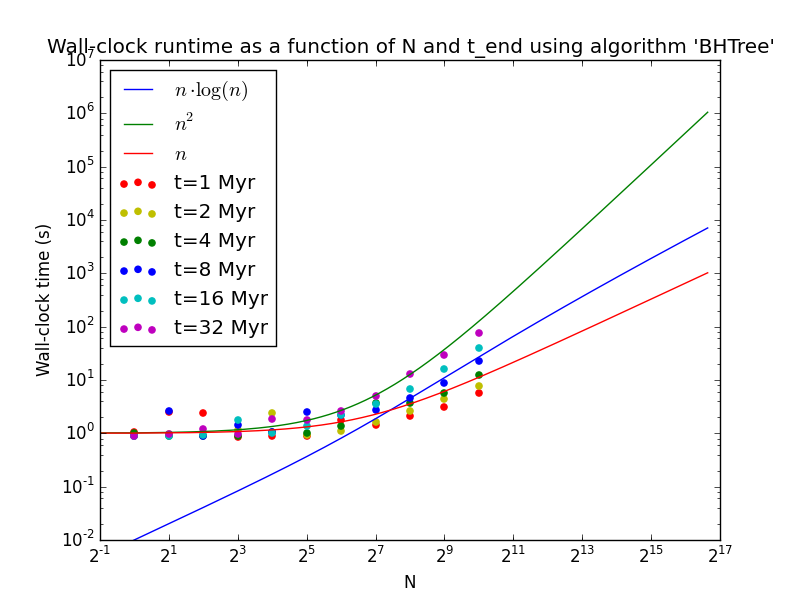
\includegraphics[width=\hsize]{img/CA_GD_TLRH_s1603221_SS_s1617451_BHTree_runtime_log_plus_O.png}
      \caption{Log-log plot of the wall-clock time as a function of both N and integration 
               end time for BHTree. Different colours indicate different end times $t_{\rm end}$ of the integration.
              }
         \label{fig:BHTree_runtime}
   \end{figure}
   
   \begin{figure}
   \centering
   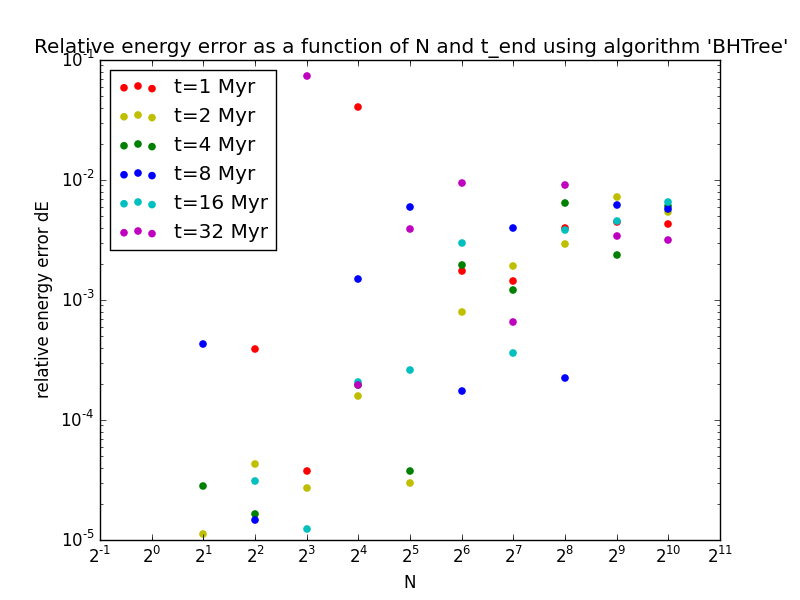
\includegraphics[width=\hsize]{img/CA_GD_TLRH_s1603221_SS_s1617451_BHTree_dE_log.png}
      \caption{Log-log plot of the relative energy error (absolute value) as a function of both N and integration 
               end time for BHTree. Different colours indicate different end times $t_{\rm end}$ of the integration.
              }
         \label{fig:BHTree_dE}
   \end{figure}
     
   \begin{figure}
   \centering
   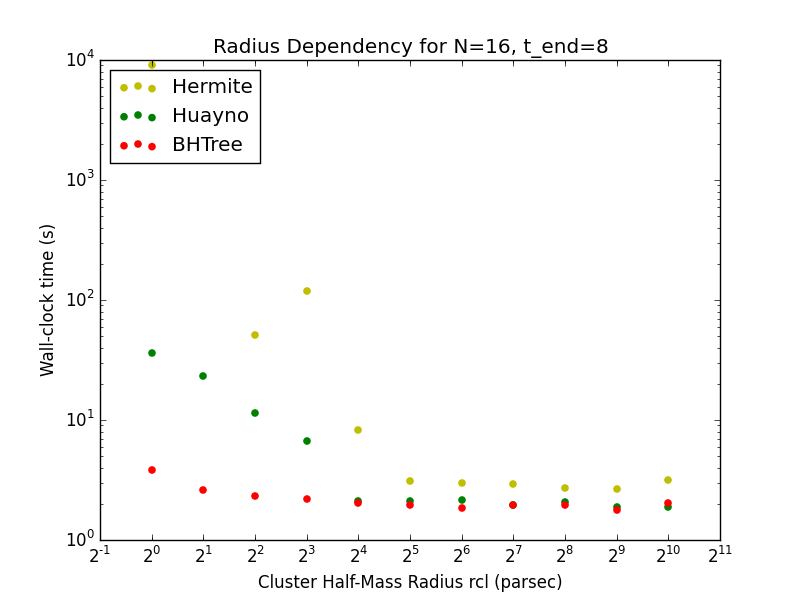
\includegraphics[width=\hsize]{img/CA_GD_TLRH_s1603221_SS_s1617451_rcldep_N16_t-end8.png}
      \caption{Wall-clock time (s) as a function of cluster half-mass radius rcl (parsec) comparison of
      	      BHTree, Huayno and Hermite algorithms for N = 8 particles, integrated until t\_end = 16 Myr.
	      Here we can see that for all three algorithms the time is constant as a function of the cluster size apart for the Hermite
	      algorithm that has an incredibly high runtime for one and two particles. For one particle the Hermite runtime is 3622 s, which is behind the legend. 
              }
         \label{fig:radius_dependency}
   \end{figure}  

The cluster size $r$ is passed to the nbody\_integrator function as parameter named `rcl'. This parameter is only used in amuse.units.nbbody\_system, which is responsible for the creation of bodies within a confined cluster with half-mass radius `rcl'. The distance between individual particles could increase  as the cluster half mass radius increases. This maximum distance between particles scales linearly with the cluster half mass radius. The distance between particles is a parameter required to calculate the force, but the number of times the force is
  calculated does not depend on it. If the cluster size increases and the number of particles is unchanged, then at a certain point in time more particles could be further away. In that case more particles will be `bundled' together in the same BHTree node, thus, in principle the calculation time could decrease as the cluster size $r$ increases if particles move further away. This prediction could be seen in Figure~\ref{fig:radius_dependency}. Moreover, it is shown that the runtime is roughly constant as a function of cluster size for the all algorithm for clusters of size greater than $2^6$ parsec. Do note that the Hermite calculation time significantly increases for lower cluster sizes. This is due to the predictor-corrector nature of the algorithm that requires significantly more steps to predict and correct when the cluster size is small. This feature of the Hermite algorithm is highly time consuming.


   \begin{figure}
   \centering
   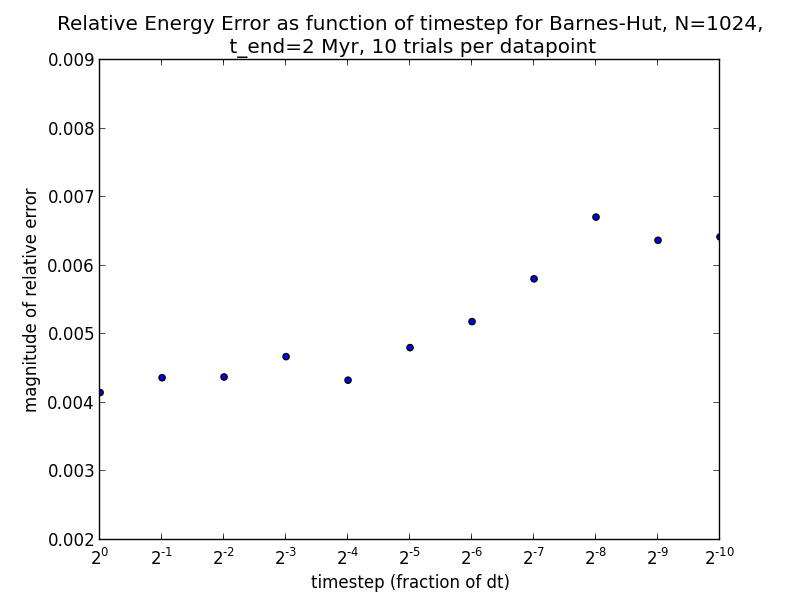
\includegraphics[width=\hsize]{img/error_for_timestep.png}
      \caption{This plot shows that for the BHTree the relative energy error (absolute value) increases as the time step decreases from 0.625 onwards. 
      	 	   All computed values are within the same order of magnitude with at most a factor of two difference between the time steps.
                    }
         \label{fig:timestep_dependency}
   \end{figure}


%__________________________________________________________________

\section{Hermite Algorithm} \label{sec:Hermite}
In this section the Hermite algorithm will be reviewed. Our methods and analysis is similar as described in Section~\ref{sec:BHTree} for the BHTree save for two noticeable differences. Firstly, we have limited our maximum number of particles considered in the analysis to 32. We have chosen to due so owing to time constrains. Where the maximum runtime for the BHTree was in the order of $10^2$, the runtime for the Hermite integrator exceeded a thousand seconds for 32 particles alone. For 1024 particles, the expected number of force calculations should be in the order of a million. Although this amount of calculations should easily lie within the abilities of modern day processing power (even on laptop computers), we found that the predictor corrector nature of the Hermite integrator produced very poor time performance. 

Secondly, we have not been able to do time step analysis as the Hermite algorithm has a variable time step scheme (see Table~\ref{tab:algorithms}). We can not tweak the performance of error by altering the time step.

The results are given in Figure~\ref{fig:Hermite_runtime} and Figure~\ref{fig:Hermite_dE}


   \begin{figure}
   \centering
   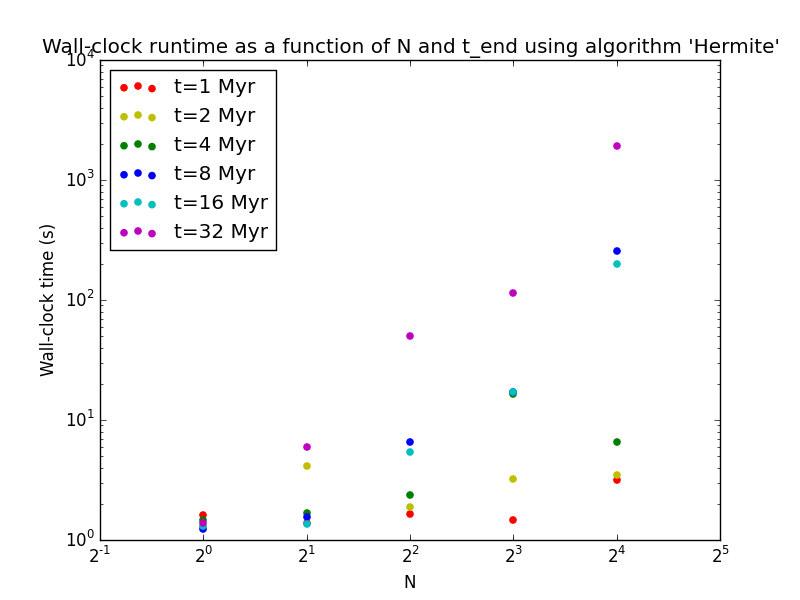
\includegraphics[width=\hsize]{img/CA_GD_TLRH_s1603221_SS_s1617451_Hermite_runtime_log.png}
      \caption{Log-log plot of the wall-clock time as a function of both N and integration 
               end time for Hermite.
              }
         \label{fig:Hermite_runtime}
   \end{figure}
   
   \begin{figure}
   \centering
   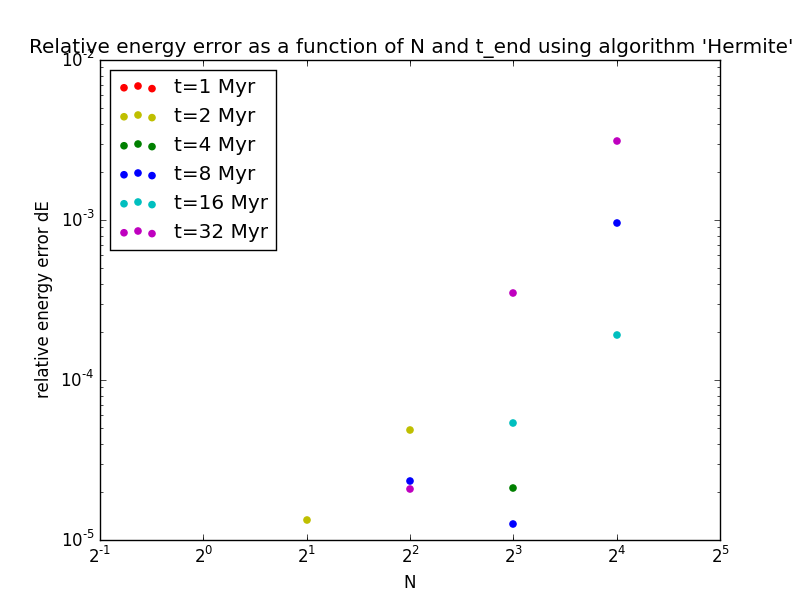
\includegraphics[width=\hsize]{img/CA_GD_TLRH_s1603221_SS_s1617451_Hermite_dE_log.png}
      \caption{Log-log plot of the relative energy error (absolute value) as a function of both N and integration 
               end time for Hermite.
              }
         \label{fig:Hermite_dE}
   \end{figure}

\section{Huayno Algorithm} \label{sec:Huayno}
In this section the Huayno algorithm will be reviewed. Our methods and analysis is similar as described in Section~\ref{sec:BHTree} for the BHTree save for one noticeable difference. Here, we have not been able to do time step analysis as the Huayno algorithm has an unknown time step scheme (see Table~\ref{tab:algorithms}). We can not tweak the performance of error by altering the time step.

The results are given in Figure~\ref{fig:Huayno_runtime} and Figure~\ref{fig:Huayno_dE}
  
   \begin{figure}
   \centering
   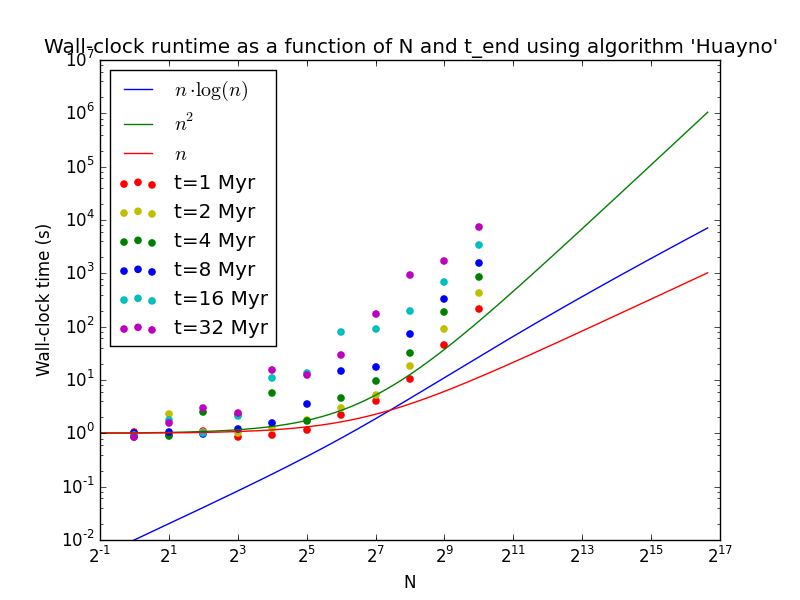
\includegraphics[width=\hsize]{img/CA_GD_TLRH_s1603221_SS_s1617451_Huayno_runtime_log_plus_O.png}
      \caption{Log-log plot of the wall-clock time as a function of both N and integration 
               end time for Huayno.
              }
         \label{fig:Huayno_runtime}
   \end{figure}
   
   \begin{figure}
   \centering
   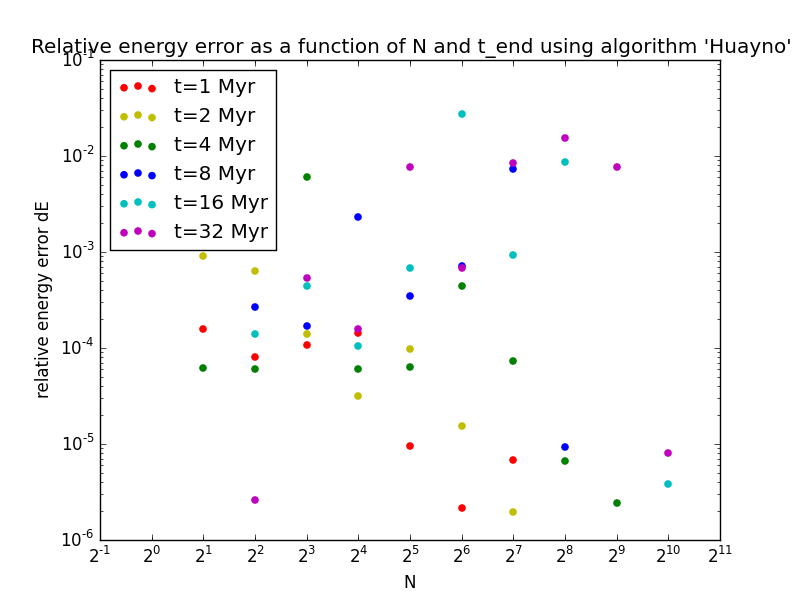
\includegraphics[width=\hsize]{img/CA_GD_TLRH_s1603221_SS_s1617451_Huayno_dE_log.png}
      \caption{Log-log plot of the relative energy error (absolute value) as a function of both N and integration 
               end time for Huayno.
              }
         \label{fig:Huayno_dE}
   \end{figure}
   


\section{Bound Cluster Mass} \label{sec:BoundClusterMass}
In this section we discuss two different methods used to determine whether a star is bound or unbound by the gravitational forces of the other stars in the galaxy working on it. Moreover, we discuss the differences between both algorithms and we conclude that the built-in is better suited for our needs.

On one hand, AMUSE has a built-in method to determine which particles are bound and unbound. This method, the HOP method \citep{1998ApJ...498..137E}, is a group-finding algorithm specifically for N-Body simulations. The algorithm works by calculating the densities at all particle positions and then following the path to the nearest particle with a higher density until the nearest particle is the particle itself. All paths of particles created this way belong to the same group if they have a shared end particle. We think the particles that are bound are all in the same group. All other particles, then, are unbound. This, however, is not clear from initial publication about the HOP algorithm.

On the other hand, we have written our own routine to calculate the bound mass. A vital assumption is that when the kinetic energy $E_{\rm kin}$ of a star is greater than the potential energy $E_{\rm pot}$, the star is unbound. Conversely, the star is bound. We have ran simulations with both algorithms, but we did not really trust the results obtained using this method. An issue arises, for instance, when simulating the galaxy in a circular orbit around a Black Hole as described in Section~\ref{sec:orbitBH_MW_Mass}. In those simulations, for every cluster size the method still returns that the galaxy is fully bound, even though our plots indicate otherwise (i.e. we can see that a significant fraction of the particles `runs away') and the HOP method yields a fully unbound galaxy. We therefore decided to use the HOP algorithm, which is available in AMUSE.
  
\section{Galaxy in Orbit around Black Hole} \label{sec:orbitBH_MW_Mass}
Here we adopt N = 1024 and we use the BHTree algorithm because it has the best time complexity. We do not adjust the default time step, as discussed in Section~\ref{sec:BHTree}. Our analysis consists of the following four parts. 

Firstly, we define a function to calculate the total bound mass of the cluster. In this case the cluster is in a system without a black hole, i.e. the function determines an intrinsic property of the cluster itself. 

Secondly, we add a black hole of mass $M = 1.26 \cdot 10^{12}$ M\Sun. Figure~\ref{fig:dvplane} shows the impact parameter $d$ versus the velocity of the cluster when it is closest to the black hole. For this we have assumed the cluster to be a point mass, since we are only interested in the behaviour of the center of mass of the cluster. We consider the cluster (point mass) bound if its velocity is smaller than the escape velocity $v_{\rm esc}$ given by \begin{eqnarray} v_{\rm esc} &= \sqrt{\frac{2 G M}{d}} \label{eq:vesc} \end{eqnarray} where $G$ is the gravitational constant (in SI), $M$ is the mass of the Black Hole and $d$ is the impact parameter.

   \begin{figure}
   \centering
   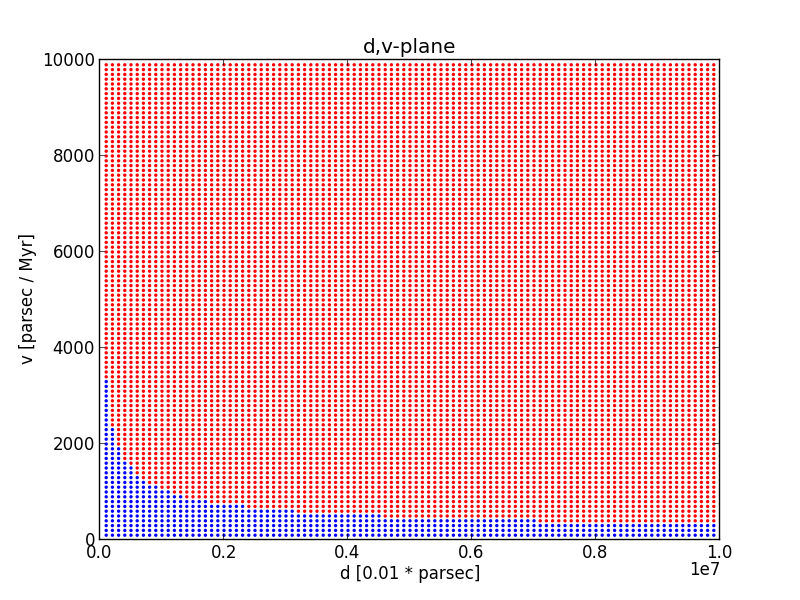
\includegraphics[width=\hsize]{img/dv_plot.png}
      \caption{Plot of the $d$,$v$-plane indicating when the cluster (simulated as a point mass) becomes bound or unbound.
      		   Red dots indicate an unbound situation, while blue dots indicate a bound situation. The black line indicates the cut off point given by
		   the escape velocity.
              }
         \label{fig:dvplane}
   \end{figure}


Moreover, we adopt a circular orbit around the black hole at a distance $R$ = 6, 12 and 18 kpc. We investigate the values of the cluster size $r$ over the distance to the Black Hole, $r/R$ to see when the cluster is bound or unbound. We simulate for $r \in [10 - 100]$ pc and added $r \in [110 - 150]$ pc for $R = 18$ kpc. The result is shown in Figure~\ref{fig:bound_mass}. Note that we used the HOP algorithm to calculate the bound mass fraction, as described in Section~\ref{sec:BoundClusterMass}. For this we first deleted the Black Hole particle out of the particle list.

Because we noticed a steep cutoff we have increased the spatial resolution for $R$ = 12 kpc between 60 pc and 80 pc, see Figure~\ref{fig:bound_mass_extra_res}. The function is not smooth but appears to contain a significant amount of noise. The most interesting behaviour of this curve is that, for all three values of $R$, the value of $r/R$ has a specific cutoff of $
 $ \mytilde 0.005 for which the cluster becomes unbound. It is around this point we are interested in expanding the parameter space to simulate.

   \begin{figure}
   \centering
   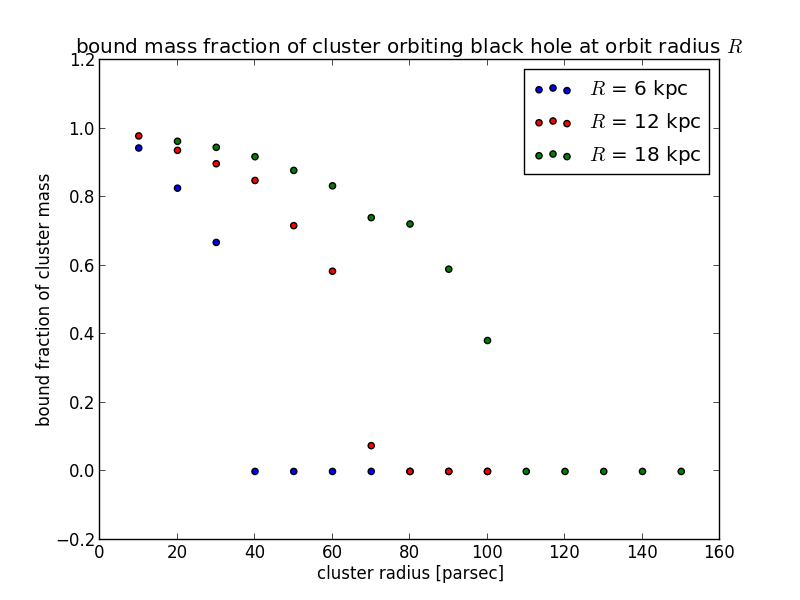
\includegraphics[width=\hsize]{img/bound_mass_at_all.png}
      \caption{Plot of the bound mass fraction as a function of the cluster radius $r$ for galaxy size $R$ = 6, 12 and 18 kpc.
      		   Note that $r/R$ has a specific value of \mytilde 0.005 for which we notice a sudden drop to zero of the bound fraction of cluster mass.
		   This behaviour is visible for all three values of $R$.
              }
         \label{fig:bound_mass}
   \end{figure}
   
  \begin{figure}
   \centering
   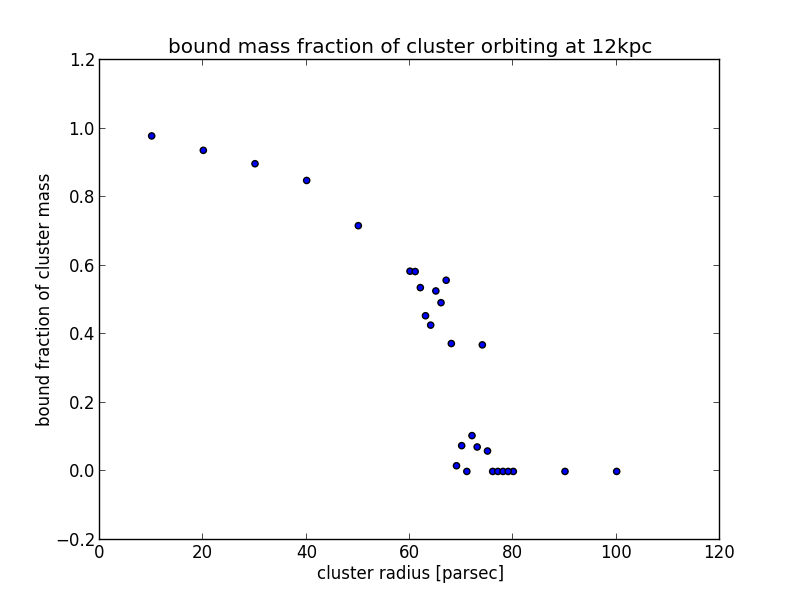
\includegraphics[width=\hsize]{img/bound_mass_at_12000_pc.png}
      \caption{Plot of the bound mass fraction as a function of the cluster radius $r$ for galaxy size $R$ =  12 kpc.
      		   Note that $r/R$ has a specific value of \mytilde 0.005 for which we notice a sudden drop to zero of the bound fraction of cluster mass.
		   We increased the spatial resolution between 60 and 80 because we noticed a steep cutoff. The function is not smooth but appears to 
		   contain a significant amount of noise around the stable/unstable border. 
              }
         \label{fig:bound_mass_extra_res}
   \end{figure}

Finally, we simulate around the bound-unbound border in the $d$,$v$-plane to obtain the mass of the post-encounter cluster and, using the Kepler package \citep{REPLACE} to calculate the orbital parameters. Table~\ref{tab:parameterspace} shows the parameter space around the bound/unbound curve used in the simulations.


   \begin{table}
      \caption[]{Parameters and results of a dozen simulations performed around the bound/unbound border. Here, $r$ is the cluster radius, $R$ the
      		    galaxy size, $v$ the velocity of the cluster, $M/M_{\rm initial}$ the bound mass fraction (post-encounter), $a$ the semi-major axis 
		    and $e$ the eccentricity.}
         \label{tab:parameterspace}
         \begin{tabular}{llllll}
            \hline
            \noalign{\smallskip}
            $r$ (pc) & $R$ (kpc) & $v / v_{\rm esc}$ & $M/M_{\rm initial}$ & a (kpc) & $e$ \\ 
            \noalign{\smallskip}
            \hline
            \noalign{\smallskip}   
            15 & 3 & 0.8 & 0.735 & 3.755 & 0.311 \\                 
            15 & 3 & 1.0 & 0.956 & 9608 & 0.999 \\
            15 & 3 & 1.2 & 0.970 & 3.409 & 1.88 \\                 
            30 & 6 & 0.8 & 0.749 & 7.649 & 0.305 \\
            30 & 6 & 1.0 & 0.922 & 2.863 $\cdot 10^4$ & 0.999 \\                 
            30 & 6 & 1.2 & 0.955 & 6.819& 1.88 \\                 
            60 & 12 & 0.8 & 0.745 & 1547 & 0.303 \\
            60 & 12 & 1.0 & 0.929 & 8.834 $\cdot 10^4$ & 0.999 \\                 
            60 & 12 & 1.2 & 0.965 & 13.64 & 1.88  \\
            90 & 18 & 0.8 & 0.767 & 22.99 & 0.305  \\
            90 & 18 & 1.0 & 0.949 & 1.398 $\cdot 10^5$ & 0.999 \\                 
            90 & 18 & 1.2 & 0.978 & 20.46 & 1.88 \\
            \noalign{\smallskip}
            \hline
         \end{tabular}
   \end{table}
         
         
         
\section{Conclusions}

   \begin{enumerate}
      \item Conlcusie 1
      \item Conclusie 2
      \item Conclusie 3
   \end{enumerate}

\begin{acknowledgements}
      The authors are grateful for the help of their supervisors
      Edwin van der Helm, MSc and Prof.dr. S.F. Portegies Zwart.
\end{acknowledgements}


%-------------------------------------------------------------------

\bibliographystyle{aa} 
%\setlength{\bibsep}{0pt} % Remove whitespace in bibliography.
\bibliography{CA_GD_TLRH_s1603221_SS_s1617451_report_aa} 
\end{document}
